\documentclass[runningheads,a4paper]{llncs}

\usepackage[utf8]{inputenc}

\usepackage{amssymb}
\setcounter{tocdepth}{3}
\usepackage{graphicx}
\usepackage{caption}
\usepackage{subcaption}

\newcommand{\keywords}[1]{\par\addvspace\baselineskip
\noindent\keywordname\enspace\ignorespaces#1}

\usepackage{pifont} 
\usepackage[utf8]{inputenc}
\usepackage{enumitem}
\usepackage[hyphens]{url}
\usepackage[pdftex,urlcolor=black,colorlinks=true,linkcolor=black,citecolor=black]{hyperref}
\def\sectionautorefname{Section}
\def\subsectionautorefname{Subsection}

% listings and Verbatim environment
\usepackage{fancyvrb}
\usepackage{relsize}
\usepackage{listings}
\usepackage{verbatim}
\newcommand{\defaultlistingsize}{\fontsize{8pt}{9.5pt}}
\newcommand{\inlinelistingsize}{\fontsize{8pt}{11pt}}
\newcommand{\smalllistingsize}{\fontsize{7.0pt}{8.0pt}}
\newcommand{\listingsize}{\smalllistingsize}%{\defaultlistingsize}
\RecustomVerbatimCommand{\Verb}{Verb}{fontsize=\inlinelistingsize}
\RecustomVerbatimEnvironment{Verbatim}{Verbatim}{fontsize=\defaultlistingsize}
\lstset{frame=lines,captionpos=b,numberbychapter=false,escapechar=§,
  aboveskip=2em,belowskip=1em,abovecaptionskip=0.5em,belowcaptionskip=0.5em,
  framexbottommargin=-1em,basicstyle=\ttfamily\listingsize\selectfont}

% use Courier from this point onward
\let\oldttdefault\ttdefault
\renewcommand{\ttdefault}{pcr}
\let\oldurl\url
%\renewcommand{\url}[1]{\defaultlistingsize\oldurl{#1}}

\usepackage[usenames,dvipsnames,svgnames,table]{xcolor}
\lstdefinelanguage{JavaScript}{
  keywords={push, typeof, new, true, false, catch, function, return, null,
    catch, switch, var, if, in, while, do, else, case, break, div, script, video},
  keywordstyle=\bfseries,
  ndkeywords={class, export, boolean, throw, implements, import, this},
  ndkeywordstyle=\color{darkgray}\bfseries,
  identifierstyle=\color{black},
  sensitive=false,
  comment=[l]{//},
  morecomment=[s]{/*}{*/},
  morecomment=[s]{<!--}{-->},  
  commentstyle=\color{darkgray},
  stringstyle=\color{green},
  morestring=[b]',
  morestring=[b]"
}
\lstset{breaklines=true}

% linewrap symbol
\usepackage{color}
\definecolor{grey}{RGB}{130,130,130}
\newcommand{\linewrap}{\raisebox{-.6ex}{\textcolor{grey}{$\hookleftarrow$}}}

% todo macro
\usepackage{color}
\newcommand{\todo}[1]{\noindent\textcolor{red}{{\bf \{TODO}: #1{\bf \}}}}

\def\JSONLD{\mbox{JSON-LD}}

\hyphenation{WebVTT}

\def\JSONLD{\mbox{JSON-LD}}

\begin{document}

\mainmatter  % start of an individual contribution

% first the title is needed
\title{Curtains Up! Lights, Camera, Action! \mbox{\enspace Documenting}~the~Creation~of~Theater~and~Opera \mbox{Productions}~with~Linked~Data~and~Web~\mbox{Technologies}}

% a short form should be given in case it is too long for the running head
\titlerunning{Curtains Up! Lights, Camera, Action!}

% the name(s) of the author(s) follow(s) next
\author{
  Thomas Steiner\textsuperscript{1}\thanks{Second affiliation: Google, Hamburg, Germany, \email{tomac@google.com}} \and
  Rémi Ronfard\textsuperscript{2}
  Pierre-Antoine Champin\textsuperscript{1} \and \\
  Benoît Encelle\textsuperscript{1}\and
  Yannick Prié\textsuperscript{3}
}
%
\authorrunning{Curtains Up! Lights, Camera, Action!}
% (feature abused for this document to repeat the title also on left hand pages)

% the affiliations are given next
\institute{
  \textsuperscript{1}CNRS, Université de Lyon, LIRIS -- UMR5205, Université Lyon~1, France\\
  \email{\{tsteiner, pierre-antoine.champin\}@liris.cnrs.fr, benoit.encelle@univ-lyon1.fr}\\
  \textsuperscript{2} Inria Grenoble Rhône-Alpes / LJK Laboratoire J. Kuntzmann - IMAGINE, France\\
  \email{remi.ronfard@inria.fr}\\
  \textsuperscript{3}CNRS, Université de Nantes, LINA -- UMR 6241, France\\
  \email{yannick.prie@univ-nantes.fr}
}

\maketitle

\begin{abstract}
For this paper, in the context of the French research project \emph{Spectacle en Ligne(s)},
we have recorded the entire set of rehearsals of one theater and one opera production
using state-of-the-art video equipment.
The resulting raw video and audio tracks as well as manually generated annotation data
were then preprocessed in order to localize actors and detect their dialogues.
Based on these preprocessing steps, we have built a~Web-based hypervideo application
that allows for navigation through performance time, performance space, and rehearsal time
using modern HTML5 Web technologies like the emerging Web Components standard.
We publish and consume the annotation data as so-called Linked Data Fragments,
a~novel way to make triple-based structured data available in a~scalable way. 
As a~direct outcome, researchers interested in the genetic analysis
and the creation process of live performances can, thanks to this application,
freely zoom in and out of scenes,
rehearsal sessions, and stage locations in order to better understand
the different steps on the way to a~chef d'œuvre.
A~live demo of the application is publicly available at the URL
\url{http://spectacleenlignes.fr/hypervideo/}.

\keywords{Hypervideo, Web Components, Linked Data Fragments, video analysis, audio analysis, theater, opera, rehearsal, live production}
\end{abstract}

\section{Introduction}

\subsection{Project Background}

The objective of the \emph{Spectacle en Ligne(s)}%
\footnote{Project website: \url{http://spectacleenlignes.fr/}} project is to create a~video corpus
of live theater and opera rehearsals and to explore the uses of this archive for
pedagogic, research, and mediation purposes.
The project is funded by the French National Agency of Research (ANR) as part of the project call
\textit{``Corpus, data and research tools in human and social sciences''}.%
\footnote{\textit{French: ``Corpus, données et outils de la recherche en sciences humaines et sociales''}}
Adopting an interdisciplinary approach, the project is structured around three complementary areas of research:
\emph{(i)}~sociological research for the study of public and existing performance archives,
\emph{(ii)}~technological research for the chained capturing and publishing of challenges of Open Access,
\emph{(iii)}~mediation research of audiences for the design of new usage scenarios of the archive.
The project ended in December 2014.

\subsection{Hypervideo Background}

The term \emph{hypervideo} is commonly used to refer to
\textit{``a~displayed video stream that contains embedded user-clickable anchors''}%
~\cite{sawhney1996hypercafe,smith2002extensible}
and annotations, allowing for navigation between the video and other hypermedia elements.
In a~2006 article in \emph{The Economist}, the authors write 
\textit{``[h]yperlinking video involves the use of ``object-tracking'' software
to make filmed objects, such as cars, clickable as they move around.
Viewers can then click on items of interest in a~video
to watch a~related clip; after it has played,
the original video resumes where it left off.
To inform viewers that a~video is hyperlinked,
editors can add highlights to moving images, use beeps as audible cues,
or display still images from hyperlinked videos
next to the clip that is currently playing''}~\cite{economist2006hypervideo}.
In standard literature, hypervideo is considered a~logical consequence
of the related concept of \emph{hypertext}~\cite{bernerslee1990hypertext}.
In contrast to hypertext, hypervideo necessarily includes a~time component,
as content changes over time.
In consequence, hypervideo has other technical and aesthetic requirements
than hypertext, the most obvious one being appropriate segmentation in scenes
or even objects.
The opportunities for feature-rich semantic hypervideos are endless,
only limited by feasibility and ease of their creation.
In this paper, we share our approach to affordably and practically document
the creation of theater and opera productions with video and Web technologies.

\subsection{Paper Contributions}

Our contributions with this paper are two-fold.
First, we show how modern HTML5~\cite{berjon2012html5} Web technologies
and the emerging Web Components~\cite{cooney2013webcomponents} standard
can be used for the documentation of theater and opera productions;
the resulting hypervideo Web Components%
\footnote{Polymer Hypervideo: \url{https://github.com/tomayac/polymer-hypervideo}}%
~\cite{steiner2014hypervideo} as well as the demo application%
\footnote{\emph{Spectacle en Ligne(s)} demo application: \url{spectacleenlignes.fr/hypervideo/}}
created for \emph{Spectacle en Ligne(s)} based thereon
are made available publicly as open source.
Second, we make use of Semantic Web technologies, namely Linked Data Fragments~\cite{verborgh2014ldf},
to publish \emph{and} consume%
\footnote{\emph{Spectacle en Ligne(s)} data portal: \url{http://spectacleenlignes.fr/query-ui/}}
the annotation data that was created during the recording phase.
This approach allows us to make our structured data reusable
by others as Linked Data~\cite{bernerslee2006linkeddata} on the one hand,
and shows its feasibility by ``eating our own dog food'' through using this data ourselves on the other.

\section{Related Work}

Related work can be regarded under the angles
of online video annotation creation, large-scale Linked Data 
efforts for video, and video documentation of theatrical performances.
Many have combined Linked Data and video,
typical examples are~\cite{lambert2010linkeddata} by Lambert \emph{et~al.}\
and~\cite{hausenblas2009im} by Hausenblas \emph{et~al.}
There are several text track enriching approaches~\cite{li2013enriching,li2012creating,yi2012synote,steiner2010semwebvid}
based on named entity recognition.
The online video hosting platform YouTube
lets publishers add video annotations
in a~closed proprietary format.
From 2009 to 2010, YouTube had a~feature called
Collaborative Annotations%
~\cite{fink2009collaborativeannotations}
that allowed video consumers to collaboratively
create video annotations.
In~\cite{vandeursen2012mediafragmentannotations},
Van Deursen \emph{et~al.}\ present a~system
that combines Media Fragments URI~\cite{troncy2012mediafragments}
and the Ontology for Media Resources~\cite{lee2012mediaontology}
in an HTML5 Web application to convert
media fragment annotations into a~WebVTT~\cite{pfeiffer2013webvtt} file
that can be used by HTML5-enabled players.
Building on their work, in~\cite{steiner2014webvtt},
we additionally allowed for writing annotations by
letting annotators create WebVTT cues with an editor.
Popcorn.js\footnote{Popcorn.js: \url{http://popcornjs.org/}}
is an HTML5 JavaScript media framework
for the creation of media mixes
by adding interactivity and context to videos
by letting users link social media, feeds,
visualizations, \emph{etc.} to moving images.
PopcornMaker%
\footnote{PopcornMaker: \url{https://popcorn.webmaker.org/}}
is an interactive Web authoring environment
allowing for videos to be annotated on a~timeline.
McAuley reports in~\cite{mcauley1994video} findings from ten years of experimentation
with recording formats and analysis for the documentation of theatrical performances.
In~\cite{lan2003video}, Lan and Morgan investigate the effects of retroactive and
focused self-monitoring through videotaping, on children's theater performance
and found that retroactive self-monitoring enhanced theater performance.
Giesekam examines in~\cite{giesekam2007staging} the use of film and video in theaters
and evaluates the impact and effectiveness of such developing multimedia technologies on practices in dramaturgy and performance.

\section{Hypervideo Web Components}
\label{sec:hypervideo-web-components}

In this section, we first provide necessary background on the emerging Web Components standard
and then describe the generic hypervideo Web Components
that were created in the context of the \emph{Spectacle en Ligne(s)} project.

\subsection{Introduction to Web Components}

Web Components is a~set of specifications, which let Web developers leverage
their HTML, CSS, and JavaScript knowledge to build widgets
that can be reused easily and reliably.\footnote{Web Components:
\url{http://www.chromium.org/blink/web-components}}
According to a~(recently discontinued) W3C Working Draft introductory document,%
\footnote{Discontinued W3C Working Draft document:
\url{http://www.w3.org/TR/2013/WD-components-intro-20130606/}~\cite{cooney2013webcomponents}}
the component model for the Web (``Web Components'') consists of five different pieces
that we will list in the following.

\begin{description}
  \item[Imports] which defines how templates, decorators and custom elements are packaged and loaded as a~resource%
  ~\cite{glazkov2014htmlimports}.
  \item[Shadow DOM] which encapsulates a~DOM subtree for more reliable composition of user interface elements%
  ~\cite{glazkov2014shadowdom}.    
  \item[Custom Elements] which let authors define their own elements, with new tag names and new script interfaces%
  ~\cite{glazkov2013customelements}.  
  \item[Decorators] which apply templates based on CSS selectors to affect rich visual and behavioral changes to documents.
  \item[Templates] which define chunks of inert markup that can be activated for use.  
\end{description}

\noindent At time of writing, partial native support for Web Components
has landed in a~number of Web browsers,
however, for the majority of browsers,
a~so-called polyfill solution is still required.
A~polyfill  is a~piece of code that provides the technology
that developers expect the browser to provide natively in the near future.
We rely on the Polymer project\footnote{Polymer project:
\url{http://www.polymer-project.org/}}
that provides Web Components support for older browsers.
Polymer allows us to create reusable widgets that introduce a~number of new
custom HTML elements for our task of hypervideo creation.

\subsection{Implementation Details}

We have developed a~number of Web Components for the creation of hypervideos.
These Web Components are behaviorally grouped together
by a~common naming convention.
In Polymer, all element names have to start with the prefix \texttt{polymer} and contain a~dash
in order to add a~namespace which avoids conflicts with existing elements.
However, this requirement is seen as a~bad practice by some,
as it makes Web Components seem like being ``owned'' by the Polymer framework.

\begin{description}
  \item[\texttt{<polymer-hypervideo>}] is the parent element of all other elements.
    It accepts the attributes \texttt{src} for specifying a~set of
    space-separated video sources (to support different encodings),
    and---analog to the native HTML5 video attributes---%
    \texttt{width} and \texttt{height} for specifying the video's dimensions,
    then \texttt{poster} for specifying the video's poster frame, and finally \texttt{muted} to specify if the video should be initially muted.
  \item[\texttt{<polymer-data-*>}] is a~set of data annotation elements
    that includes the two shorthand annotation types
    \texttt{<polymer-data-actor>} for annotating video actors and
    \texttt{<polymer-data-overlay>} for annotating visual overlays,
    and the generic \texttt{<polymer-data-annotation>} for other annotations.
  \item[\texttt{<polymer-track-*>}] are the two elements
    \texttt{<polymer-track-chapters>} and \texttt{<polymer-track-subtitles>},
    which rely on WebVTT~\cite{pfeiffer2013webvtt} text tracks
    of the types ``chapters'' and ``subtitles'' that they enrich with
    automatically generated chapter thumbnails and a~full text subtitle view.
  \item[\texttt{<polymer-visualization-*>}] currently provides the
    following two visualization elements
    \texttt{<polymer-visualization-timeline>} on the one hand and 
    \texttt{<polymer-visualization-toc>} on the other
    that create a~timeline view and a~table of contents
    that put all encountered \texttt{<polymer-track-*>}
    and \texttt{<polymer-data-*>} elements in a~temporal context.
\end{description}

\noindent We have made an online demo application available at
\url{http://hypervideo.herokuapp.com/demo.html} that showcases these Web Components
and recall that we share their implementation as open source.
As both native Web Component support in Web browsers and the Polymer project
are constantly evolving and still in flux, the demo currently works best on
the latest versions of the Chrome browser.
A~screenshot of the application can be seen in \autoref{fig:screenshot},
the corresponding underlying code sample is shown in \autoref{listing:polymer}.
These components communicate with each other through standard JavaScript events,
so when a~components needs to communicate its state to another, \emph{e.g.},
\texttt{<polymer-hypervideo>} the current time of the video to one of the
visualization components like the \texttt{<polymer-visualization-timeline>},
it fires an event that components can subscribe to and react upon.
\autoref{listing:events} shows the relevant code snippets.

\begin{figure}[htb!]
  \centering
  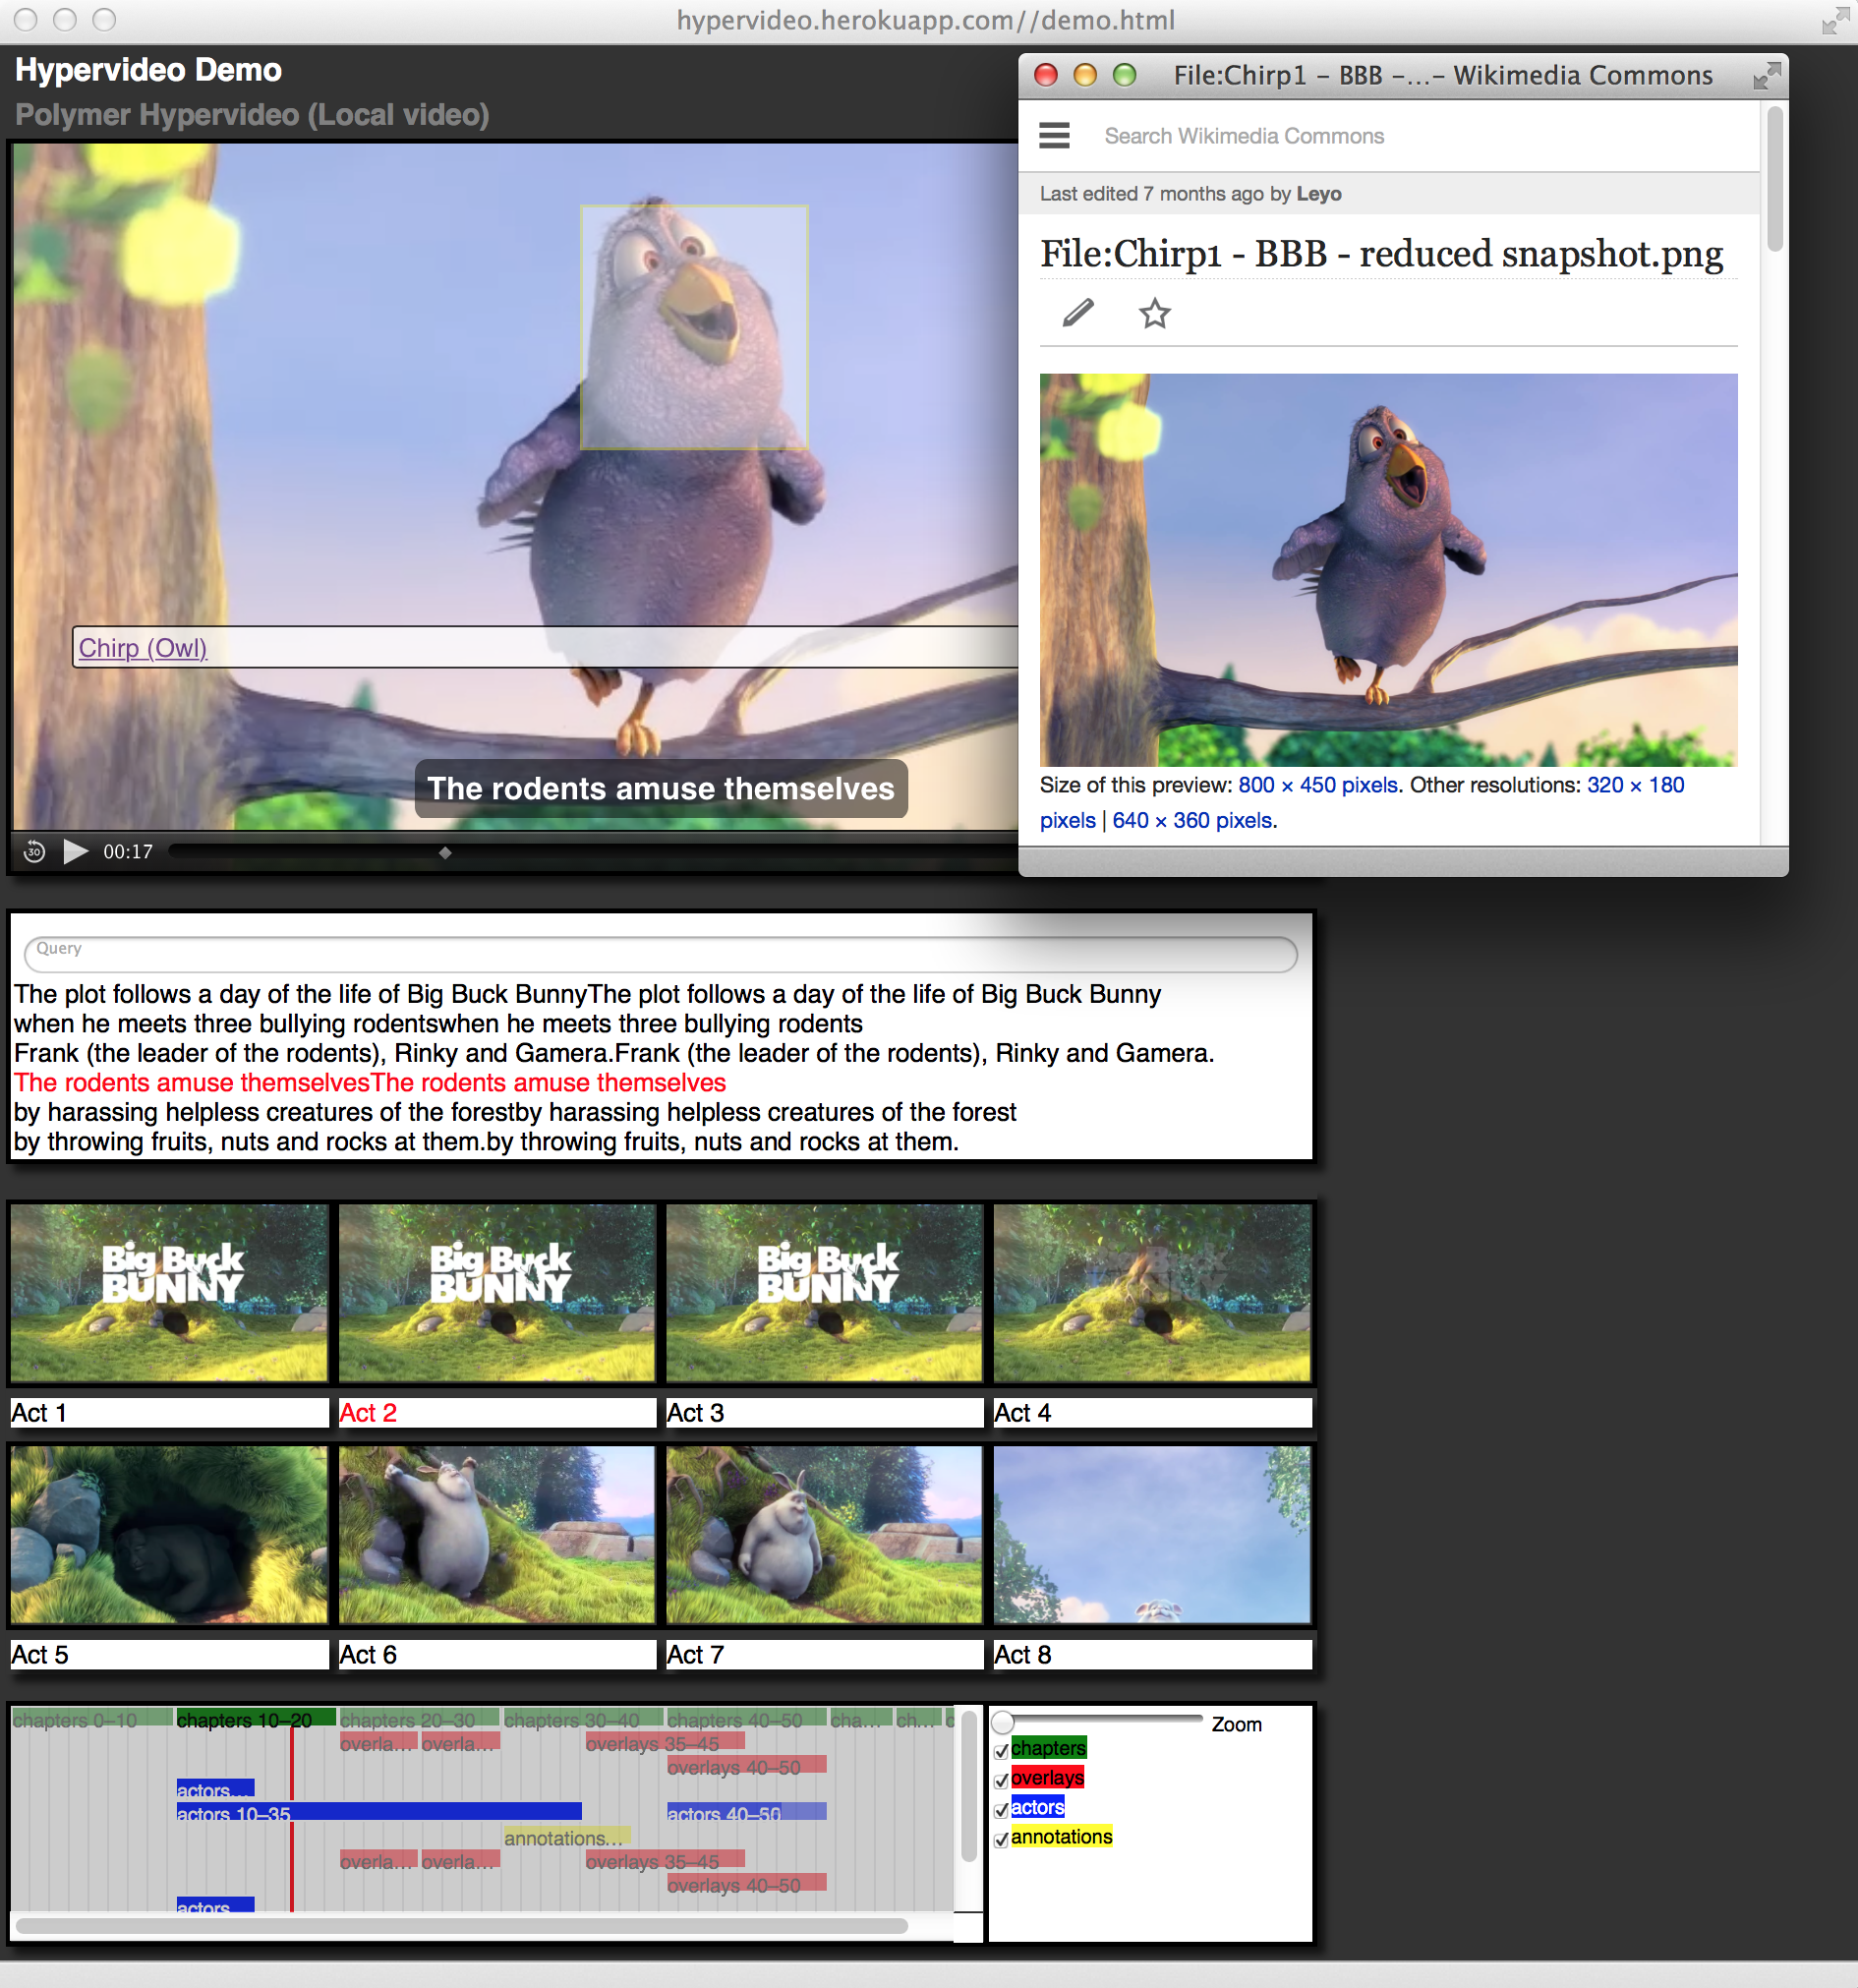
\includegraphics[width=0.95\linewidth]{screenshot}
  \caption{Generated hypervideo based on the mark-up in \autoref{listing:polymer},
  including subtitles, chapters, timeline, and table of contents;
  the actor annotation contains a~spatial fragment~\cite{troncy2012mediafragments}
  (owl's head) and a~link
  to a~Wikimedia Commons page}
  \label{fig:screenshot}
\end{figure}

\begin{lstlisting}[caption={Web Components mark-up for the hypervideo in \autoref{fig:screenshot}, including subtitles, chapters, timeline, and table of contents; the actor annotation contains a~spatial fragment
(\texttt{xywh})~\cite{troncy2012mediafragments} and a~link (\texttt{url})
  to Wikimedia Commons},
  label=listing:polymer, language=xml,
  float=b!, stringstyle=\color{gray},morekeywords={polymer,hypervideo,track,subtitles,chapters,toc,timeline,visualization,data,actor,src,end,start,name,url,width,height,muted,displaysubtitlesgroup,orientation,displaychaptersthumbnails,xywh}]
<polymer-hypervideo src="big_buck_bunny.mp4 big_buck_bunny.webm"
     width="400" height="225" muted>
    
  <polymer-data-actor start="10" end="35" name="Chirp (Owl)" xywh="170,20,70,80" 
       url="http://commons.m.wikimedia.org/wiki/File:Chirp1_-_BBB_-_reduced_snapshot.png">
  </polymer-data-actor>

  <polymer-track-subtitles src="subtitles.vtt" displaysubtitlesgroup>
  </polymer-track-subtitles>

  <polymer-track-chapters src="thumbs.vtt" displaychaptersthumbnails>
  </polymer-track-chapters>

  <polymer-visualization-timeline orientation="landscape">
  </polymer-visualization-timeline>
  
</polymer-hypervideo>
\end{lstlisting}

\begin{lstlisting}[caption={Native JavaScript event communication
  between Web Components},
  label=listing:events, language=JavaScript,
  float=b!, stringstyle=\color{gray},morekeywords={addEventListener,document}]
// === In polymer-hypervideo.js: ===
// listen to native html5 video timeupdate events
video.addEventListener('timeupdate', function() {
  that.currentTime = video.currentTime;
  // publish hypervideotimeupdate events
  that.fire('hypervideotimeupdate', { currentTime: that.currentTime });
});


// === In polymer-visualization-timeline.js: ===
// listen to hypervideotimeupdate events
document.addEventListener('hypervideotimeupdate', function(e) {
  var currentTime = e.detail.currentTime;
  // update the time marker
});
\end{lstlisting}

\subsection{Evaluation of the Web Components Design Choice}

The creation of new Web Components is a~not too difficult task
for an experienced Web developer.
Especially Polymer's \texttt{<seed-element>}%
\footnote{Polymer \texttt{<seed-element>}:
\url{https://www.polymer-project.org/docs/start/reusableelements.html}}
makes getting started straight-forward.
The biggest challenge and at the same time the biggest chance
is the dynamic nature of Web Component development.
Support for Web Components has partially landed natively in Web browsers,
which means the polyfill has to do less and less work emulating native support.
Existing bugs are generally fixed in a~timely manner in the frequent new releases of Polymer.
Communication between Web Components can be subject to race conditions,
as event listeners may not yet have been created at the time an event is being sent.
Especially with dynamically created Web Components this can be an issue,
also across browsers.
We had to introduce short timeouts for certain Web Components
before they propagate their properties up to their parent Web Component.
Concluding, Web Components were nevertheless the right design choice.
The ease of use of the finished Web Components (see \autoref{listing:polymer})
and the fact that Web Components can be created and interacted with using JavaScript
(see \autoref{listing:events} and \autoref{listing:ldfclientcode})
just like regular HTML elements greatly outweigh the initial development efforts
as we will show in more detail \autoref{sec:evaluationo-of-the-demo-application}.


\section{Linked Data Publication and Consumption}
\label{sec:linked-data-publication-and-consumption}

In this section, we first introduce the concept of Linked Data
and Tim Berners-Lee's Linked Data principles,
and then Ruben Verborgh's Linked Data Fragments.
This finally leads us to the \emph{Spectacle en Ligne(s)} Linked Data portal.

\subsection{Introduction to Linked Data}

Linked Data~\cite{bernerslee2006linkeddata} defines a~set of agreed-on
best practices and principles for interconnecting and publishing structured data on the Web.
It uses Web technologies like the Hypertext Transfer Protocol~\cite{fielding1999http}
and Unique Resource Identifiers (URIs,~\cite{bernerslee2005uri})
to create typed links between different sources.
The portal \url{LinkedData.org} defines Linked Data as being
``about using the Web to connect related data that wasn't previously linked,
or using the Web to lower the barriers to linking data currently linked using other methods.''
Tim Berners-Lee defined the four rules for Linked Data in a~W3C Design Issue as follows.

\begin{enumerate}
	\item Use URIs as names for things.
	\item Use HTTP URIs so that people can look up those names.
	\item When someone looks up a~URI, provide useful information, using the standards (RDF, SPARQL).
	\item Include links to other URIs, so that they can discover more things.
\end{enumerate}

Linked Data uses the Resource Description Framework (RDF,~\cite{klyne2004rdf})
to create typed links between things in the world.
The result is often-times referred to as the Web of Data.
RDF encodes statements about things in the form of triples that take the form subject, predicate, object. 
In this context, Heath and Bizer~\cite{bizer2009linkeddatastory} also speak of RDF links,
\emph{i.e.}, dereferencing the URI that appears as the destination of a~link
yields a~description of the linked resource in question.

\subsection{Linked Data Fragments}
Various access mechanisms to Linked Data exist on the Web,
each of which comes with its own trade-offs regarding query performance, freshness of data,
and server cost/availability.
To retrieve information about a~specific subject, you can dereference its URL.
SPARQL~\cite{prudhommeaux2008sparql} endpoints allow to execute complex queries on RDF data,
but they are not always available.
While endpoints are more convenient for clients, individual requests
are considerably more expensive for servers.
Alternatively, a~data dump allows interested parties to query locally.
However, especially with dynamic datasets, data dumps risk to get outdated quite quickly.
Users then always have to download the entire updated data dump again
or work with data diffs.
Linked Data Fragments~\cite{verborgh2014ldf} provide a~uniform view
on all such possible interfaces to Linked Data,
by describing each specific type of interface by the kind of fragments through which
it allows access to the dataset.
Each fragment consists of three parts that we will list in the following.

\begin{description}
	\item[data:] all triples of this dataset that match a~specific selector;
	\item[metadata:] triples that describe the dataset and/or the Linked Data Fragment;
	\item[controls:] hypermedia links/forms that lead to other Linked Data Fragments.
\end{description}

This view allows to describe new interfaces with different trade-off combinations.
One such interface is triple pattern fragments~\cite{verborgh2014triplepatterns},
which enables users to host Linked Data on low-cost servers with higher availability
than public SPARQL endpoints, or even for free~\cite{matteis2014ldf}
on consumer cloud storage products.
Such a~light-weight mechanism is ideal to expose mid-size datasets on commodity hardware
in a~scalable and ad hoc manner using triple pattern fragments.

\subsection{Linked Data Portal}

We use the Linked Data Fragments server implementation Server.js%
\footnote{Server.js: \url{https://github.com/LinkedDataFragments/Server.js}} by Ruben Verborgh.
Installing the server requires Node.js 0.10 or higher and is tested on OSX and Linux.
We also make a~browser interface available that is based on the Linked Data Fragments
client implementation Browser.js%
\footnote{Browser.js: \url{https://github.com/LinkedDataFragments/Browser.js}} by Ruben Verborgh.
We expose the data at the URL \url{http://spectacleenlignes.fr/query-ui},
which is host to a~user interface that allows for SPARQL queries to be executed.
A~screenshot of the query interface can be seen in \autoref{fig:ldf}.

\subsection{Linked Data Fragments Web Component}

Verborgh's original \texttt{ldf-client} library was written for a~Node.js environment.
We have compiled it using browserify,%
\footnote{Browserify: \url{http://browserify.org/}}
a~tool that allows modules designed for Node.js to be used from a~Web browser context.
This allows us to query our Linked Data portal from a~browser context using a~declarative Web Component
called \texttt{<polymer-ldf-client>}%
\footnote{\texttt{<polymer-ldf-client>}:
\url{https://github.com/tomayac/polymer-ldf-client}}
that we have also released as open source.
The HTML markup of a~Web Component that allows for declaratively accessing the data in the Linked Data portal is depicted in \autoref{listing:ldfclient},
the JavaScript source code for obtaining streaming and polling data
is shown in \autoref{listing:ldfclientcode}.

\begin{lstlisting}[caption={Linked Data Fragments Web Component \texttt{<polymer-ldf-client>}},
  label=listing:ldfclient, language=XML,
  float=b!, showstringspaces=false, stringstyle=\color{gray},morekeywords={polymer,ldf,id,client,responseFormat,query,startFragment}]
<polymer-ldf-client
   id="polymer-ldf-client-streaming"
   responseFormat="streaming"
   query="SELECT DISTINCT ?frag WHERE {
      ?a a &lt;http://advene.org/ns/cinelab/ld#Annotation&gt; ;
        &lt;http://advene.org/ns/cinelab/ld#hasFragment&gt; ?frag ;
        &lt;http://advene.org/ns/cinelab/ld#taggedWith&gt;
          [ &lt;http://purl.org/dc/elements/1.1/title&gt; 'personnages: Maggie'],
          [ &lt;http://purl.org/dc/elements/1.1/title&gt; 'personnages: Brick'];
        .
     }"
   startFragment="http://spectacleenlignes.fr/ldf/spectacle_en_lignes">
 </polymer-ldf-client>
\end{lstlisting}

\begin{lstlisting}[caption={Obtaining streaming and polling data from the Linked Data Fragments Web Component \texttt{<polymer-ldf-client>}},
  label=listing:ldfclientcode, language=JavaScript,
  float=b!, showstringspaces=false, stringstyle=\color{gray},morekeywords={document,addEventListener,alert,querySelector,querySelectorAll}]
var ldfClient = document.querySelector('#polymer-ldf-client-streaming');

/* Streaming example */

// Process data as it appears
ldfClient.addEventListener('ldf-query-streaming-response-partial', function(e) {
  alert(e.detail.response);
});

// Get notified once all data is received
ldfClient.addEventListener('ldf-query-streaming-response-end', function() {
  alert('Received all data');
});


/* Polling example */

// Poll for data
ldfClient.addEventListener('ldf-query-polling-response', function(e) {
  alert(e.detail.response);
});

// Manually trigger data polling
var button = document.querySelector('#button');
button.addEventListener('click', function() {
  ldfClient.showNext();
});
\end{lstlisting}

\begin{figure}[hbt]
  \centering
  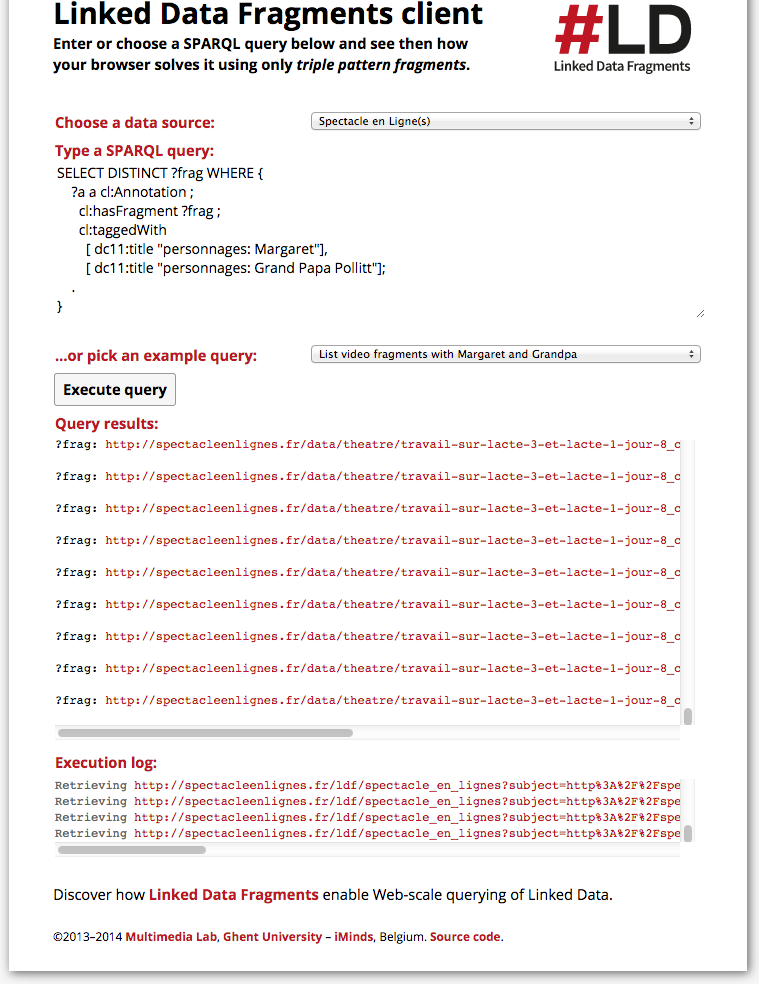
\includegraphics[width=1\textwidth]{linkeddatafragments.png}
  \caption{Linked Data portal for the project \emph{Spectacle en Ligne(s)}: \url{http://spectacleenlignes.fr/query-ui/}}
  \label{fig:ldf}
\end{figure}

\subsection{Evaluation of the Linked Data Fragments Design Choice}

Linked Data Fragments turned out to be a~good design choice.
Our mid-size dataset fits the use case perfectly well.
Building upon Linked Data Fragments' promise to keep the server simple
and enable smart clients, we can support complex queries on our dataset
even on commodity hardware.
While the processing speed may not in all cases compete with a~performant
native SPARQL query engine, the streaming nature of Linked Data Fragments
results delivery allows the user to see and process partial results as they come,
or simply to wait for the complete result.
Our \texttt{<polymer-ldf-client>} Web Component supports both kinds of operation
through a~\texttt{responseFormat} attribute.

\section{The \emph{Spectacle en Ligne(s)} Demo Application}

We recall the objective of the \emph{Spectacle en Ligne(s)} project,
which  is to create a~video corpus of live theater and opera rehearsals
and to explore the uses of this archive for pedagogic, research, and mediation purposes.
The demo application should facilitate the navigation through performance time,
performance space, and rehearsal time of the recorded œuvres.
It was built on top of the hypervideo Web Components
that were introduced in \autoref{sec:hypervideo-web-components}
and uses the project's Linked Data portal described in
\autoref{sec:linked-data-publication-and-consumption} through a~dedicated Web Component.
From the recording phase, we have several video tracks for each rehearsal day
as well as WebVTT text tracks and manual annotations from the preprocessing phase.
Manual annotations mainly contain act and scene data, sparse mise en scène data,
and in some cases information on the acting persons in a~particular scene.

\subsection{Data Flow}

Starting with a~list of all available videos
(the demo application does not contain the full list of all recordings),
we first obtain the relevant WebVTT text track for the selected video
and via JavaScript create an empty \texttt{<polymer-hypervideo>} container.
The text track is of type chapters (see~\cite{pfeiffer2013webvtt} for available types)
and is converted to a~\texttt{<polymer-track-chapters} element
that gets appended to the \texttt{<polymer-hypervideo>} container.
We interpret chapters as text cues in the œuvres, which allows us to navigate directly into them.
All chapters from the \texttt{<polymer-track-chapters} element are automatically displayed
on a~dynamically inserted \texttt{<polymer-visualization-timeline>} element.
In continuation, we then query the Linked Data portal for all annotations available for this video
using a~dynamically inserted \texttt{<polymer-ldf-client>} Web Component.
Incoming annotations are converted to \texttt{<polymer-data-annotation>} elements
that are then placed on the \texttt{<polymer-visualization-timeline>} element.
Finally, we obtain a~WebVTT text track of type subtitles (again see~\cite{pfeiffer2013webvtt})
that contains the spoken text of each text cue of the œuvre in the video in question.
We dispose of HTML documents of the recorded œuvres
that show the text and mise en scène instructions in a~human-friendly way.
Using common CSS selectors, we identify text cues in this document and align them
with the text cue data from the WebVTT subtitles text track.
This allows us to visually highlight text cues in the human-friendly documents
upon cue change events that are sent by the \texttt{<polymer-hypervideo>} element.
\autoref{fig:demoapp} shows all Web Components and the human-readable documents in action
for three different iterations.

\subsection{Enabled Navigation Patterns}

As outlined earlier, we have several videos for each rehearsal day.
Actors rehearsed the acts of each œuvre on different days
and not necessarily in chronologically correct order.
In the simplest form, we allow for consuming the videos in sequential order
to revive the rehearsal days and to see act by act, scene by scene, text cue by text cue
how the actors and the metteur en scène worked on them.
Each annotation, represented through yellow blocks in the timeline beneath the video
in \autoref{fig:demoapp}, acts as a~hyperlink
that makes the video jump right to the annotation's time code.
The same holds true for the chapter annotations that represent the text cues,
displayed as green blocks in the timeline.
Most interesting to the user probably is the navigation by text cue,
where the user can see how a~certain text cue evolved over time.
\autoref{fig:demoapp} shows act 1, cue 7.9 on three different days,
starting with the first lecture of the text at a~table on day~1,
over to an early rehearsal on day~8 on a~private stage,
and ending with the technical mise en scène on day~40 on the public stage.
Upon mouse-over on the main video, a~hovering semi-transparent navigation control gets displayed
that lets the user navigate to the next or previous rehearsal day,
or the next or previous text cue.
Additionally, three select boxes on top of the main video allow for focused
by-text-cue, by-video, and by-rehearsal-day navigation.

\subsection{Evaluation of the Demo Application}
\label{sec:evaluationo-of-the-demo-application}

Through our groundwork with the hypervideo and Linked Data Fragments Web Components, 
building the final application was a~rather straight-forward task.
All that was missing was the application logic that orchestrates the different Web Components.
The whole application required no more than 500 lines of JavaScript code.%
\footnote{\emph{Spectacle en Ligne(s)} demo application:
\url{https://github.com/tomayac/postdoc/tree/master/demos/polymer-hypervideo/spectacle-en-lignes}}
As we make all source codes of the involved Web Components and the application itself available,
future reuse of our work in other theater or opera performances is rendered possible.
The opera and theater partners of the \emph{Spectacle en Ligne(s)} project
particularly appreciated the complete freedom of navigation in the whole recording archive.
By dissolving the temporal order of the rehearsals in the application,
they could analyze and study the progress of the different scenes, acts,
and even text cues on a~level of detail not seen before. 

\begin{figure}
        \centering
        \begin{subfigure}[b]{\textwidth}
                \centering
                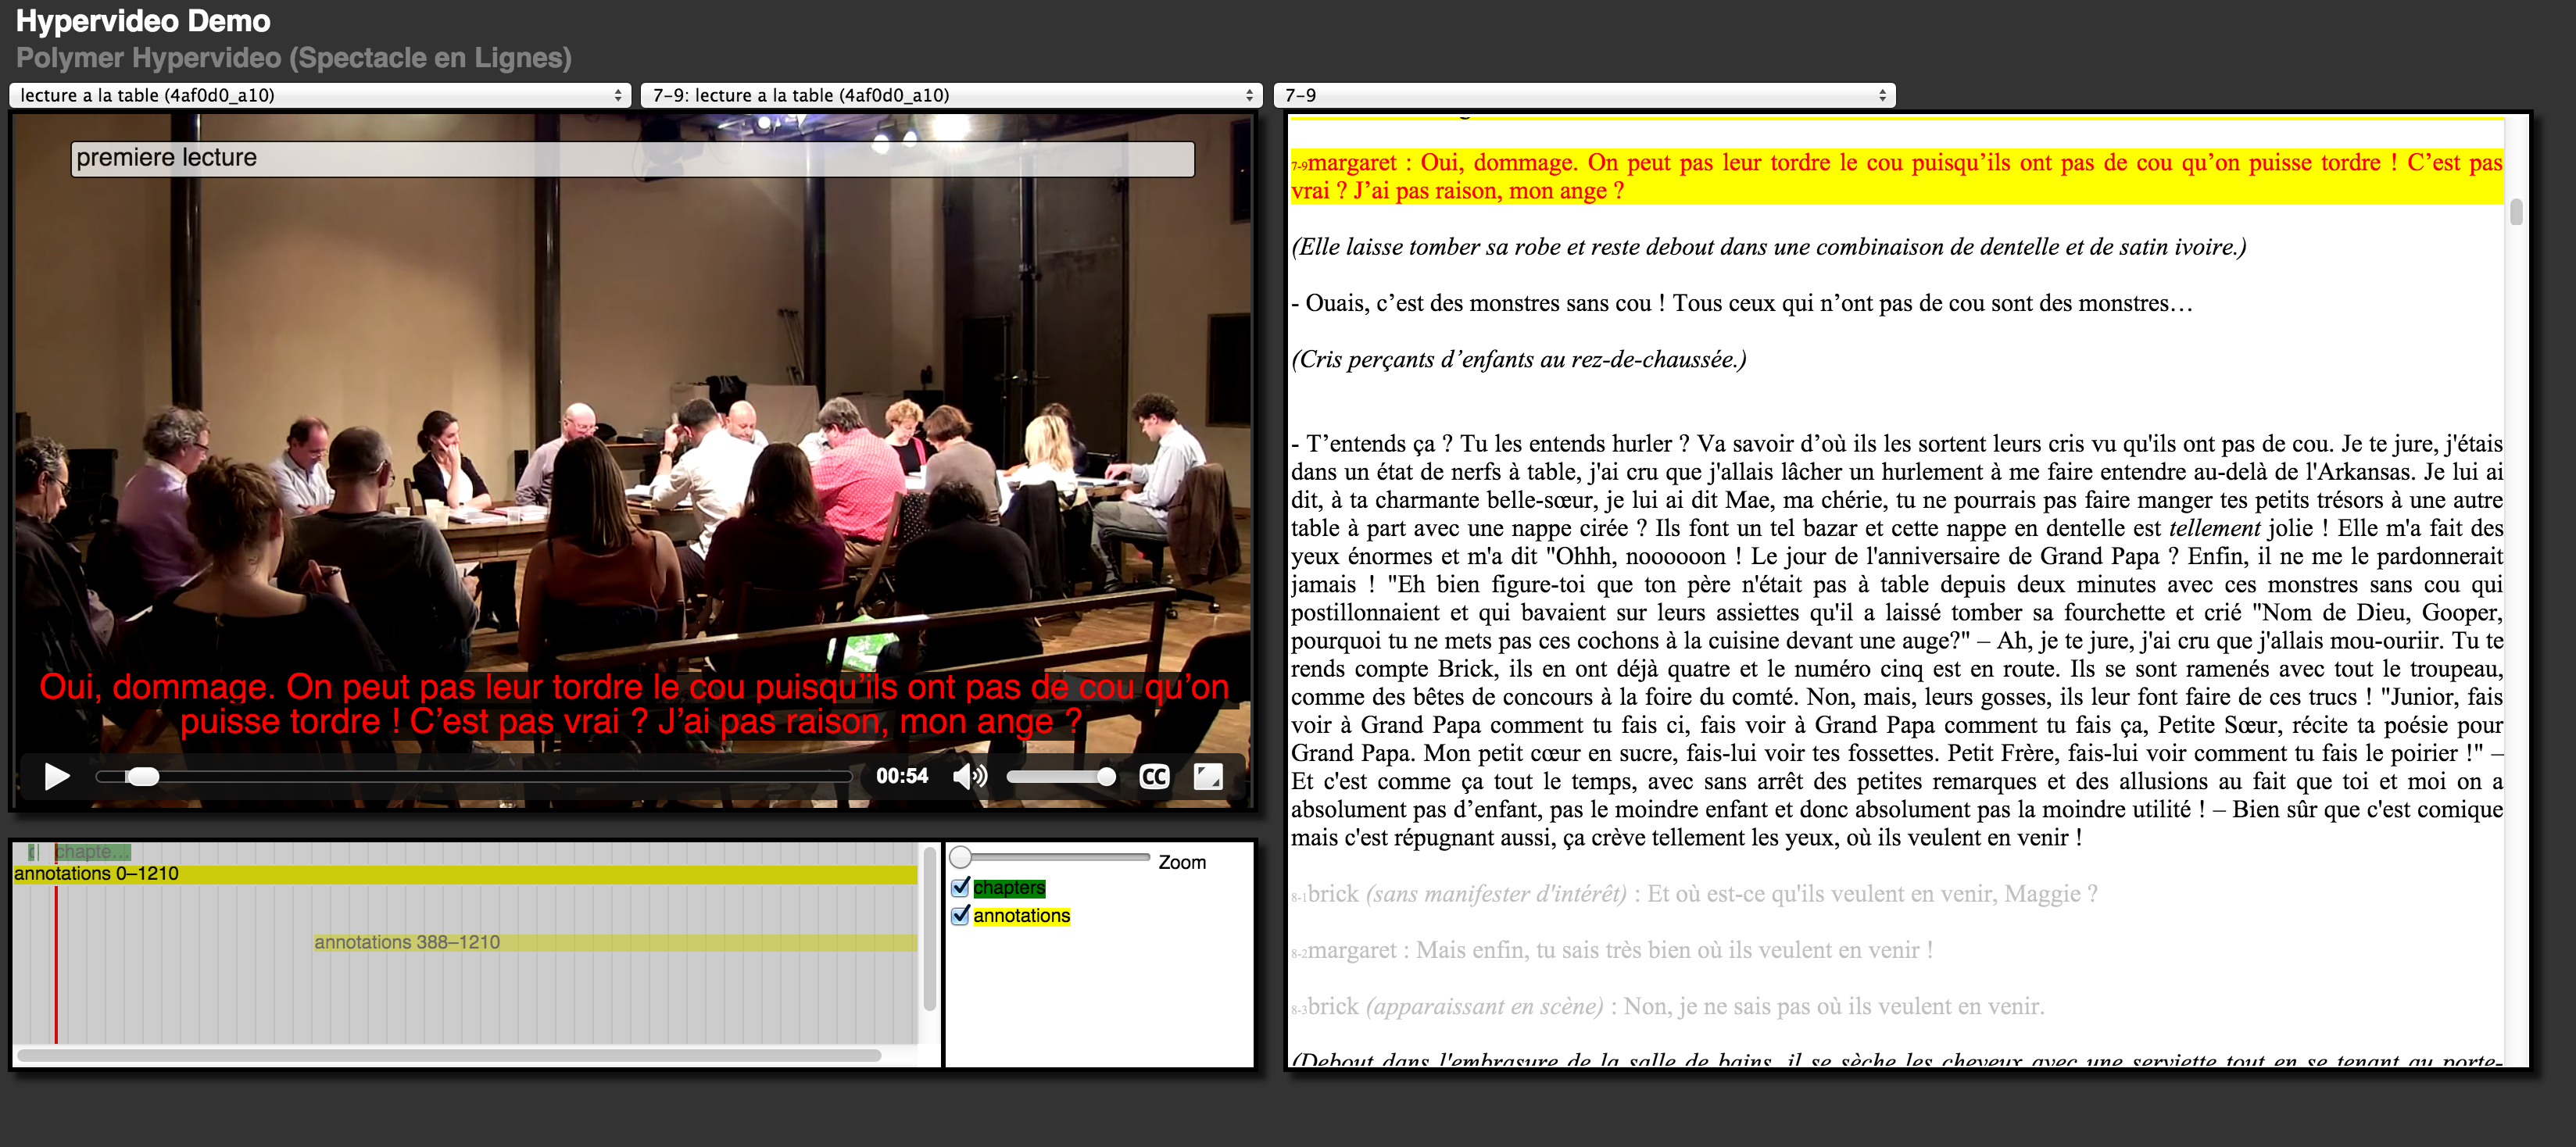
\includegraphics[width=0.9\textwidth]{spel1}
                \caption{Day~1, first lecture at the table,
                	\url{http://spectacleenlignes.fr/hypervideo/\#lecture-a-la-table_4af0d0_a10/7-9}}
                \label{fig:day1}
        \end{subfigure}
        
        \begin{subfigure}[b]{\textwidth}
                \centering
                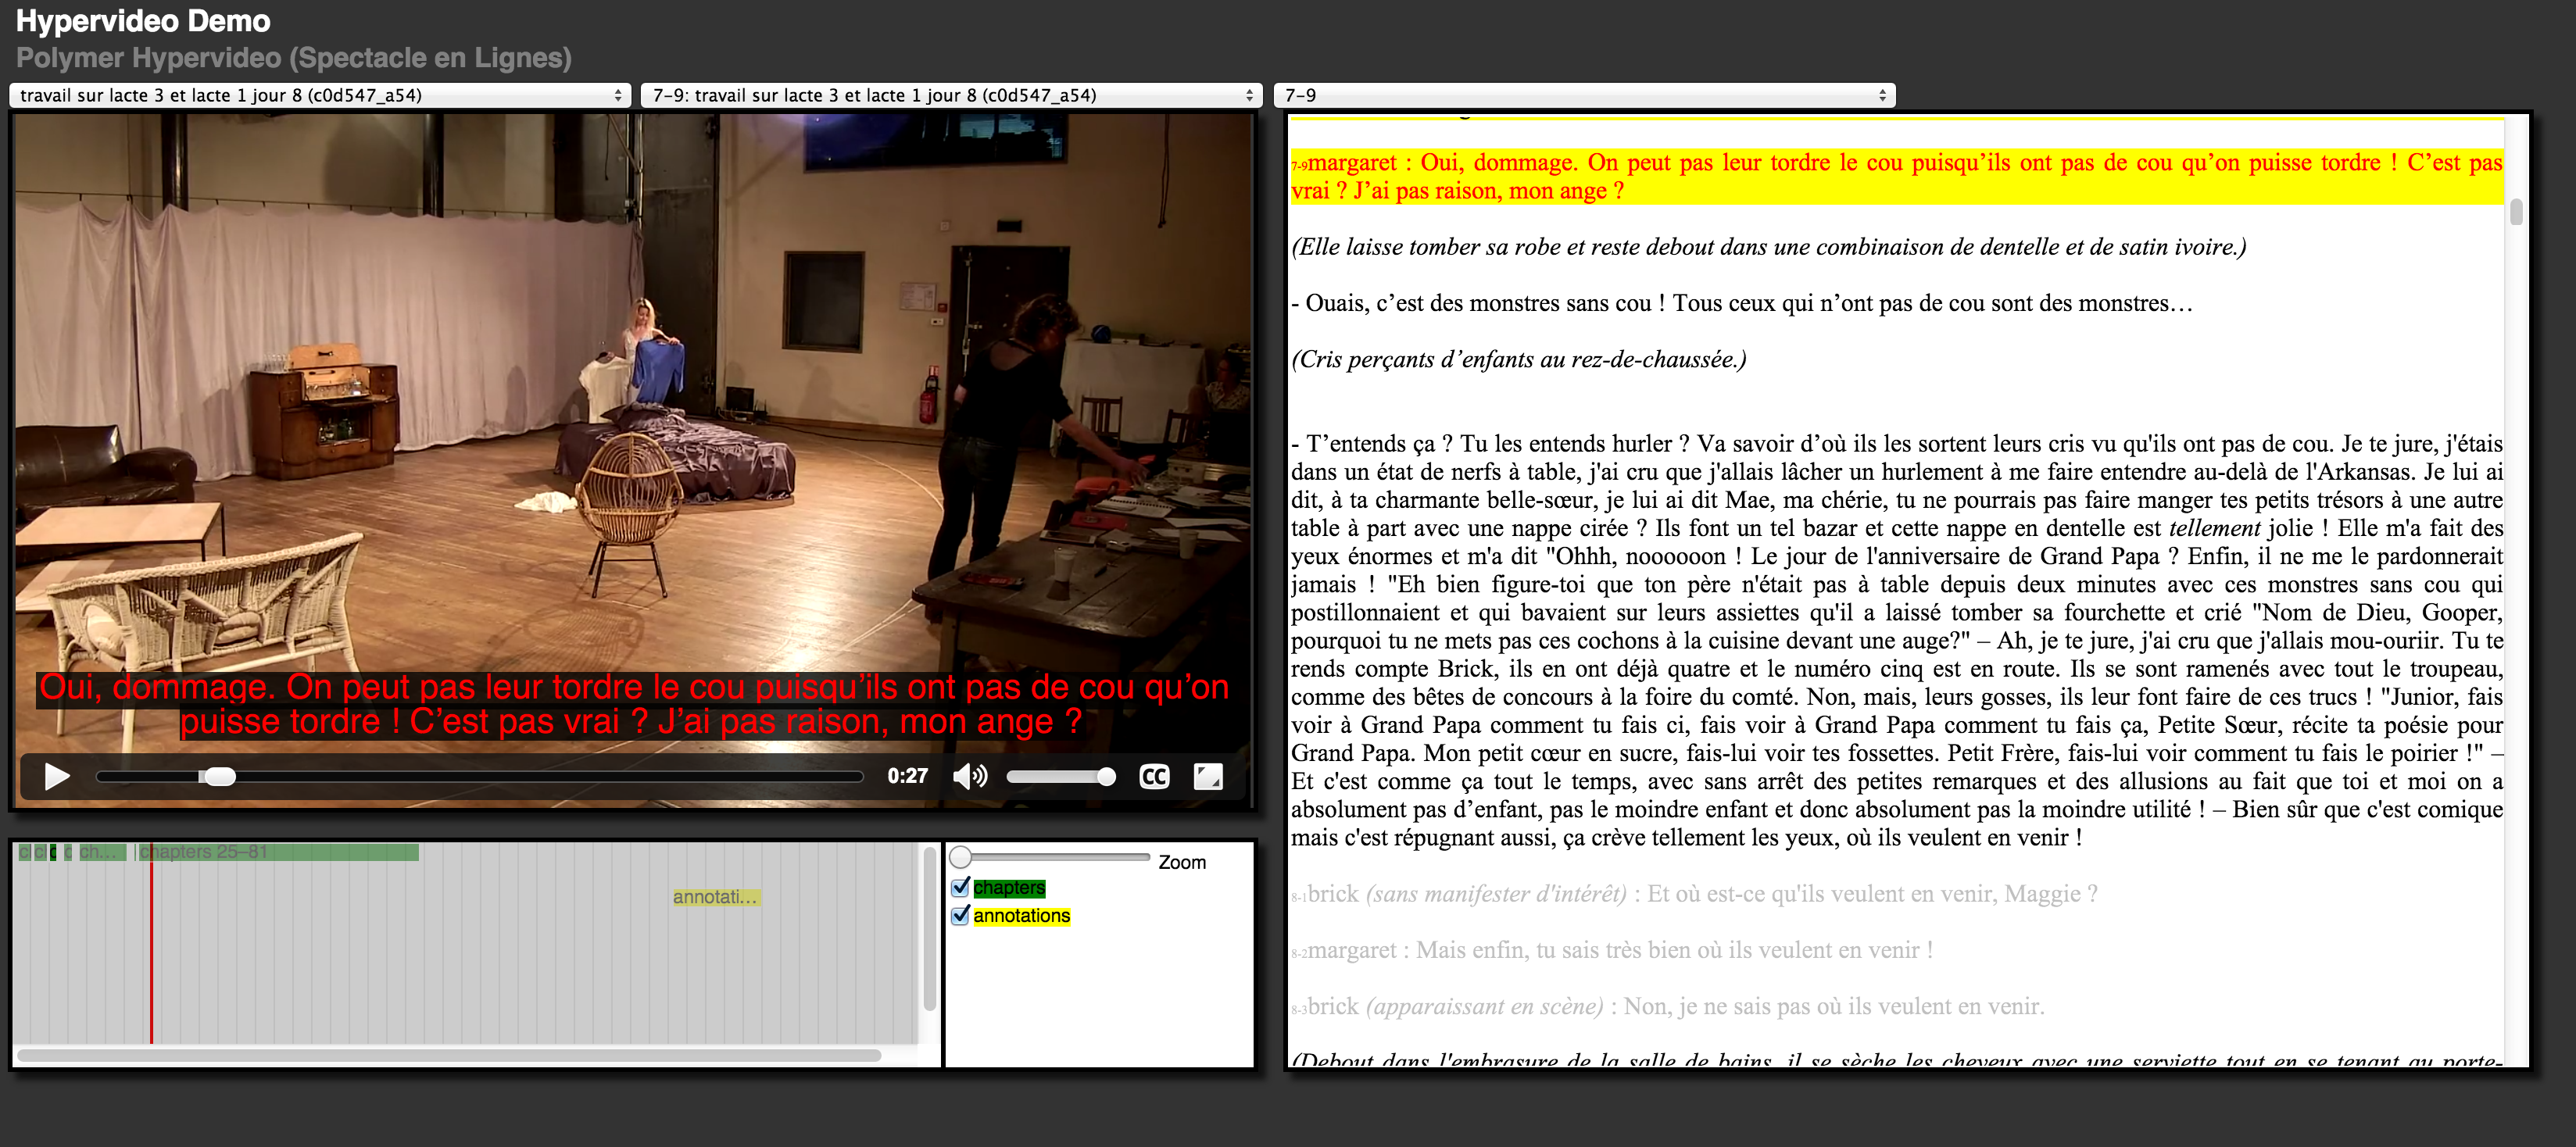
\includegraphics[width=0.9\textwidth]{spel2}
                \caption{Day~8, rehearsals of act~1,
                	\url{http://spectacleenlignes.fr/hypervideo/\#travail-sur-lacte-3-et-lacte-1-jour-8_c0d547_a54/7-9}}
                \label{fig:day8}
        \end{subfigure}
        
        \begin{subfigure}[b]{\textwidth}
                \centering
                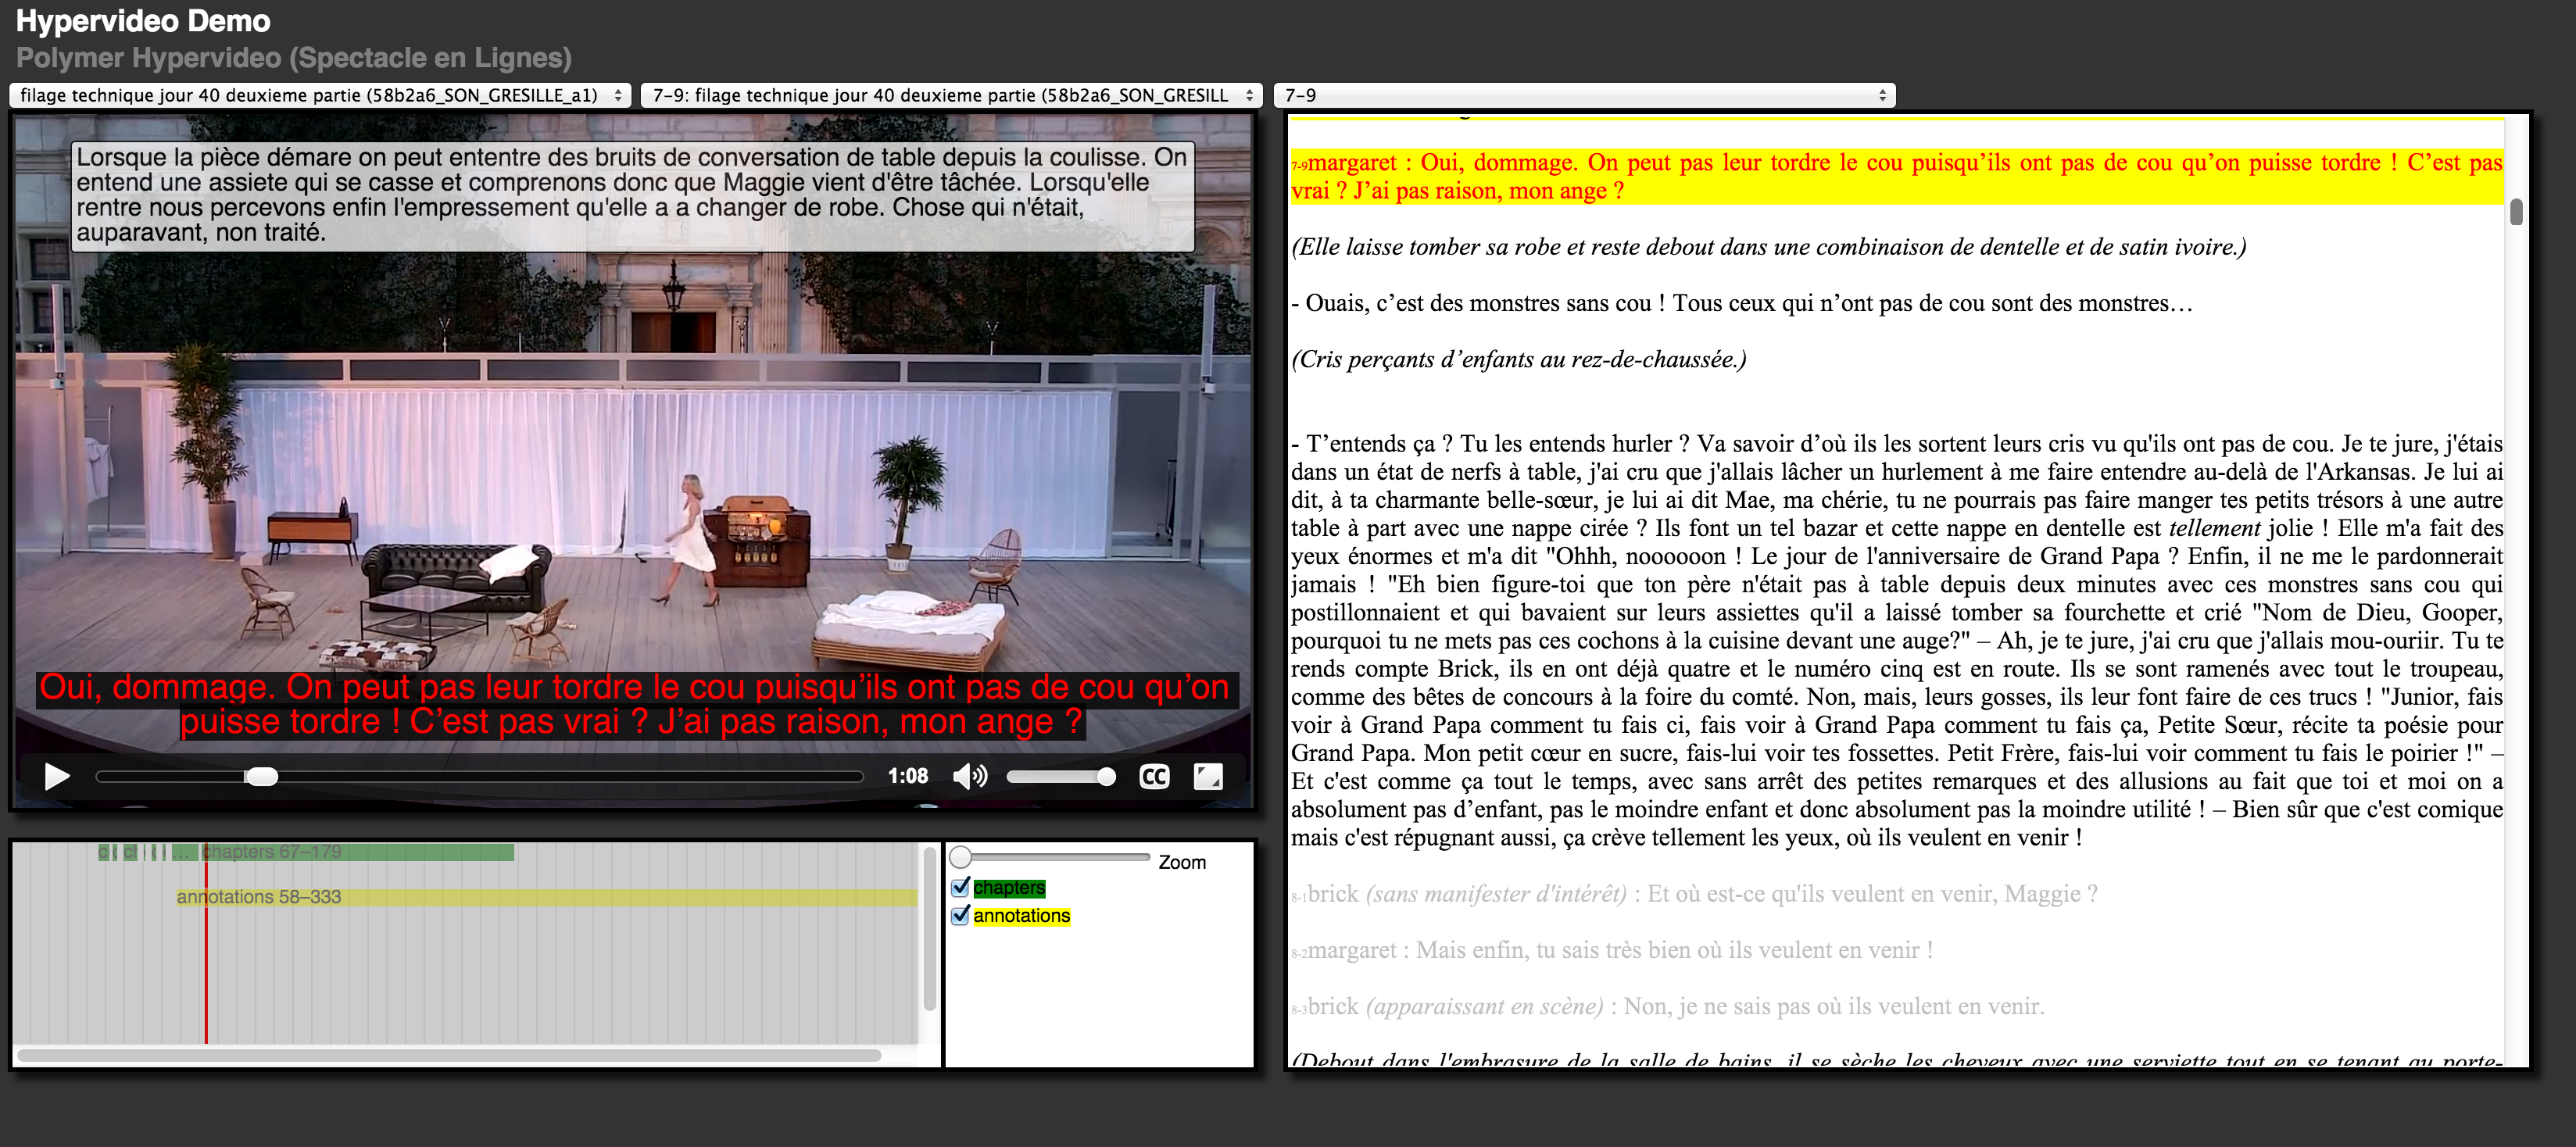
\includegraphics[width=0.9\textwidth]{spel3}
                \caption{Day~40, technical mise en scène,
                	\url{http://spectacleenlignes.fr/hypervideo/\#filage-technique-jour-40-deuxieme-partie_58b2a6_SON_GRESILLE_a1/7-9}}
                \label{fig:day40}
        \end{subfigure}
        \caption{Evolution of act~1, cue 7.9 of T. Williams' \emph{Chatte Sur Un Toit Brulant}}\label{fig:demoapp}
\end{figure}

\section{Conclusions and Future Work}

In this paper, we have first described the objectives of our project \emph{Spectacle en Ligne(s)}.
Second, we have introduced the concept of hypervideo, followed by a~look at related works
in the areas of online video annotation creation, large-scale Linked Data efforts for video,
and video documentation of live theatrical and musical performances.
In continuation, we provided necessary background on the emerging Web Components standard.
As the first contribution of our paper, we have implemented and evaluated hypervideo Web Components
that can be used to create hypervideos in a~declarative way through nothing but custom HTML tags.
Objects or temporal points of interest in the hypervideos can be annotated,
such annotations then appear on an interactive timeline.
We have then looked at Linked Data sharing principles and introduced Linked Data Fragments
as an appropriate way to share our annotation data for others
and ourselves to consume in a~scalable manner.
The second contribution is a~Web Component that allows for interacting with Linked Data Fragments
in a~streaming or polling way again purely declaratively.
Finally, we have combined all generated Web Components in a~demo application
that showcases the power and simplicity of our approach.
The source codes of all involved Web Components and the application itself
are available as open source to encourage broad reuse.

Future work will mainly concentrate on the hypervideo Web Components.
We will evaluate their usefulness for further use cases like,
for example, Web video courses and improve them accordingly if necessary.
As we have repeatedly expressed, the Web Components standard is still in flux.
As more and more Web browsers will gain native support for Web Components,
existing timing challenges that we encountered occasionally will be resolved.
Work on more hypervideo features has already started like camera selection
or inter-hypervideo communication for synchronized hypervideo experiences.
On the Linked Data side, we want to further improve the retrieval speed
of Linked Data Fragments in our Web Component by allowing for parallel multiplexed query requests.

Concluding, we are content of how far the limits of the Web have been pushed.
Tasks like hypervideo creation were a~thing of native applications
that did not allow for their results to be easily shared on the Web.
Through our hypervideo Web Components, creating a~basic hypervideo
has become accessible enough that standard Web developers can do it.
The promise of Linked Data in the end are synergies between data that was not interlinked before.
By following Linked Data principles and thanks to our Linked Data Fragments Web Component,
these synergies can be reached in the context of a~Web application with very reasonable effort,
as we have shown in this paper.
We encourage others to reuse our Web Components in their own applications
and to further extend and improve them.
We cannot wait to see what they will create.

\begin{center}
  ---
  Curtains down. And cut.	
\end{center}



\bibliographystyle{abbrv}
\bibliography{references}
\end{document}
